\documentclass[12pt,a4paper]{journal}
\usepackage[margin=1in]{geometry}

\usepackage{times}

\usepackage[utf8]{inputenc}
\usepackage[T1]{fontenc}
\usepackage{indentfirst}
\usepackage{amsmath}
\usepackage{amsfonts}
\usepackage{amssymb}
\usepackage{caption}
\usepackage{subcaption}
\usepackage{graphicx}
\usepackage{siunitx}
\sisetup{range-phrase=--, range-units=single}

\graphicspath{{img/}}
\usepackage[numbers, super, sort&compress]{natbib}


\usepackage{tcolorbox}

\begin{document}

\section*{\textit{In Silico} Clinical Trials in the Retina}

The previous sections have detailed the vast literature that deals with modelling retinal haemodynamics, oxygenation, and the impact of drugs in both healthy and diseased retinas. However, there is currently very little research on formalising these models within the framework of in silico clinical trials (ISCTs). ISCTs are effectively simulations of clinical trials to test medical devices or drugs with the aim of eventually being used as digital evidence to reduce, refine and replace animal and human participants in preclinical and clinical experiments~\cite{Viceconti2021a}. At each stage of clinical trials (preclinical, Phase I, II, III), ISCTs can be used: for early proofs-of-concept in the drug development phase; to simulate greater numbers of patients in each phase hence representing greater biological variability in the trial; to augment trials such that fewer real-world patients are required; to run numerous trials that can optimise the intervention that wouldn’t be possible in reality; as well as to investigate rare events that might not occur in a real-world trial~\cite{Pappalardo2019, ICKT105, Viceconti2017}. Another crucial aspect of an ISCT is the ability for a patient to act as their own control simulation-wise, introducing a new potentially more impactful/patient-specific way of running clinical trials.

The paradigm of an ISCT is very similar to that of a real-world clinical trial except the disease, intervention and trial setup is simulated. ISCTs require virtual populations of the disease of interest; a mechanistic model of the disease and treatment using the proposed intervention; and a statistical analysis plan that will analyse the output of the trial~\cite{Alfonso2020}. Figure~\ref{fig:ISCT} depicts a general schematic of how an ISCT might run for nAMD drug testing.

\begin{figure}[h]
  \centering
  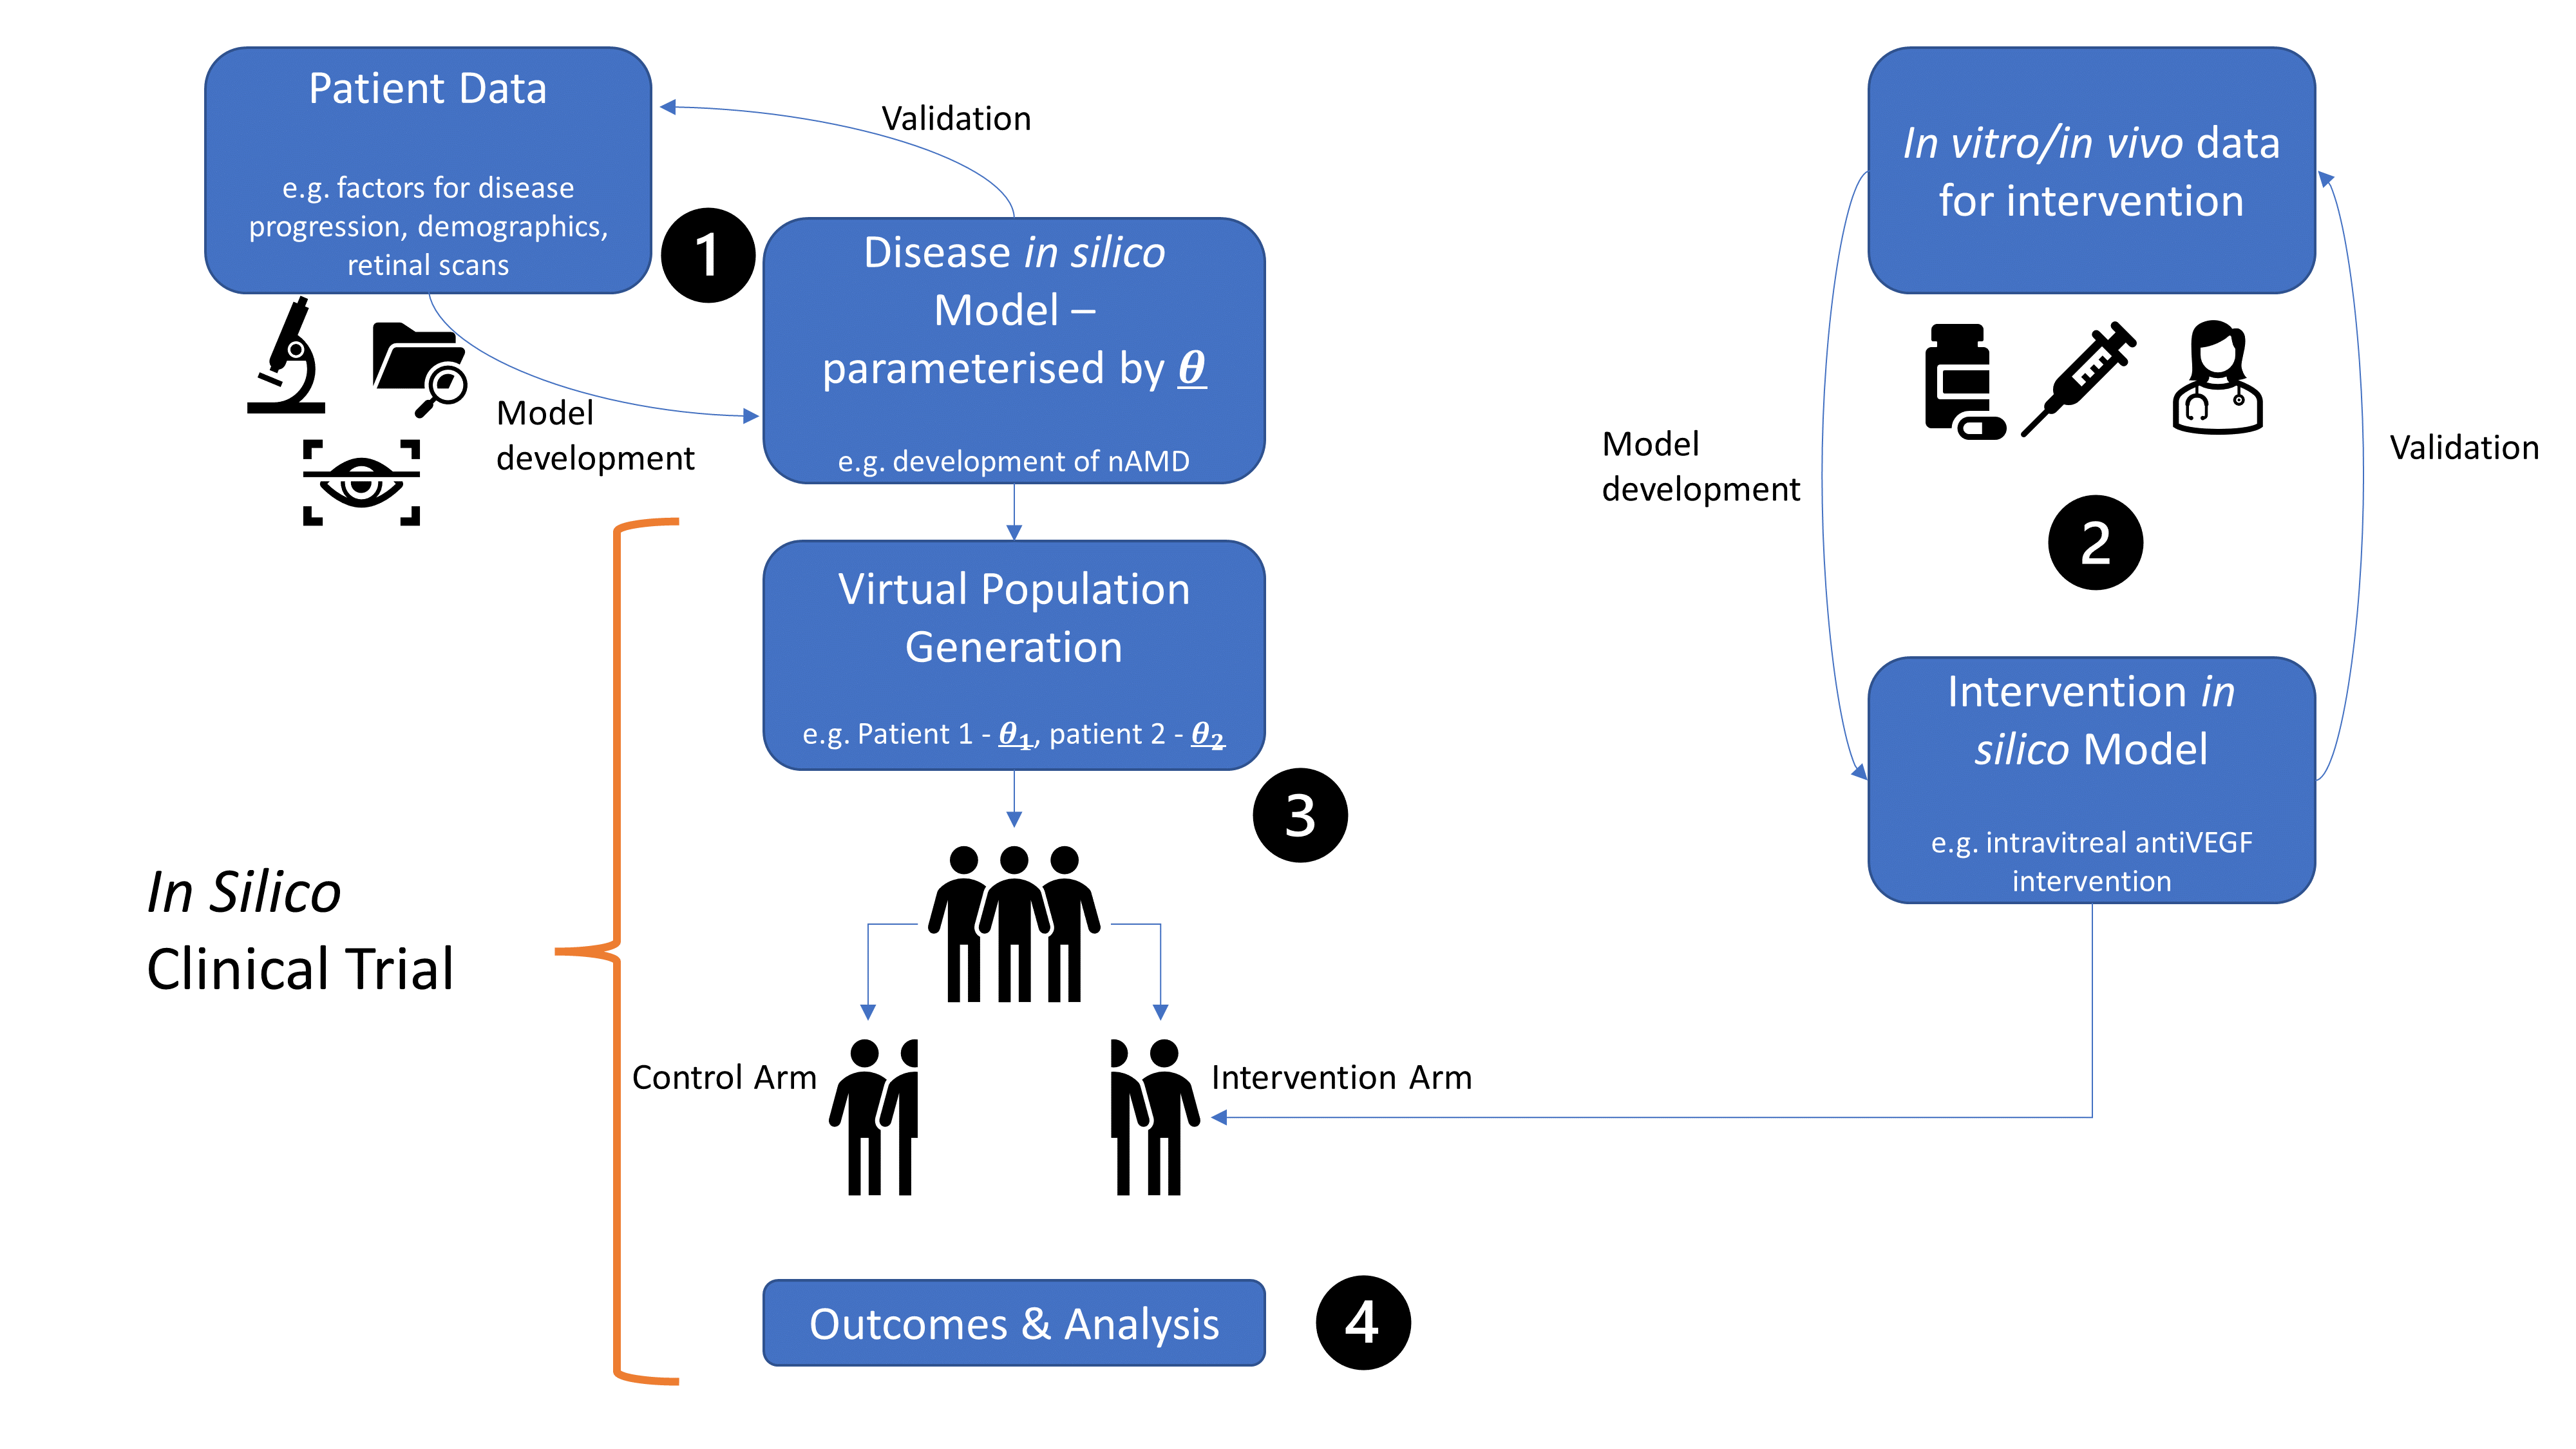
\includegraphics[width=1\textwidth, height=9.3cm]{Fig_sec_8.png}
  \hfill
  \caption{Schematic of a generic ISCT with an example of nAMD drug testing. 1) \textit{In silico} model development of disease with validation loop linked to patient data. 2) \textit{In silic} model development of intervention with validation loop linked to \textit{in vitro} and \textit{in vivo}. 3) Virtual population generation using the disease model parameters. 4) ISCT run on intervention and control arms with appropriate outcomes and analysis.}
  \label{fig:ISCT}
\end{figure}

\subsection*{Mechanistic models of disease and intervention}

The central aspect of any ISCT is the mechanistic model that predicts the outcome of an intervention (or lack thereof). This is equivalent to the administration of the intervention in a real-world clinical trial. The mechanistic model is one that is based on the underlying physics and chemistry of the system being investigated. This model will usually simulate a disease, for example cancer tumour growth~\cite{Jenner2021}. The intervention is then also simulated, in this case oncolytic viruses that can target the tumour cells. Both the disease model and intervention model must be validated against \textit{in vitro} or \textit{in vivo} data in order to be used in an ISCT (Figure~\ref{fig:ISCT}).

Examples of disease/intervention models that have been developed include coronary stent models for occlusive heart diseases~\cite{Antonini2021, Berti2021}, insulin control algorithms in Type 1 diabetes~\cite{Kovatchev2009}, non-pharmaceutical interventions on respiratory tract interventions~\cite{Arsene2022}, bone morphogenetic treatment in paediatric orphan bone disease~\cite{Carlier2018}, anaemia treatment in haemodialysis patients~\cite{Fuertinger2018}, warfarin in atrial fibrillation patients~\cite{Ravvaz2017}, cancer vaccines on lymph node cancers~\cite{Gaffney2022}, targeted delivery of drugs in patients with covid-induced pneumonia~\cite{Wang2022}, mematine treatment of Alzheimer’s disease~\cite{Swietlik2022}, flow diverters in intracranial aneurysms~\cite{SarramiForoushani2021}, predicting pro-arrhythmic cardiotoxicity in cardiomyocytes~\cite{Passini2017}, and thrombectomy/thrombolysis for acute ischaemic stroke~\cite{Konduri2020}, amongst many more.

Within this review, we have also demonstrated the vast literature on \textit{in silico} models of retinal disease, ranging from non-neovascular AMD and retinitis pigmentosa (Section 6), to neovascular AMD and diabetic retinopathy (Section 5), as well as models of intervention through intravitreal injections, implants, and sub-retinal injections (Section 7). This has laid the groundwork to adapt these models into the ISCT paradigm. Despite the rapidly growing literature on ISCTs in various disease conditions, little or no papers have been published on applying this paradigm to diseases of the retina.

Once a mechanistic model of disease and intervention has been established and extensively validated, the next step is to generate virtual populations with this disease that can be used in the ISCT.

\subsection*{Virtual Populations}

To run clinical trials, populations of the target population are required. A crucial first step is therefore to generate virtual populations (VPs) of the disease of interest that will eventually be used in the \textit{in silico} clinical trials. For example, if an intervention for nAMD patients will be tested \textit{in silico}, a population of nAMD patients is required.

Virtual population generation is a nascent and rapidly developing field. In essence, a virtual patient is one with a specific set of parameters for a given disease model. Virtual populations are therefore sets of patients with parameters that reproduce the statistics of interest of the clinical population of interest~\cite{Allen2016}.

One simple method of generating VPs is to assume a Gaussian distribution for each model parameter that will be patient specific~\cite{Gaffney2022, Jenner2021}. The mean and standard deviation of the parameters can be adjusted to match empirically observed data either manually or through optimization~\cite{Alfonso2020}. Often, these patient parameters are not independent of each other – for example, sex and height are correlated. Therefore, more complex sampling strategies that maintains the relationships between patient parameters have been developed.

Bayesian statistics have been used extensively to generate patient parameter populations for the purpose of ISCTs. Haddad et al. generated VPs using a Bayesian framework for augmenting clinical trials, demonstrating decreased sample size and trial length would be required for the real-world trial when using these VPs~\cite{Haddad2017a}. For warfarin patients, a Bayesian model was used to generate VPs from a pre-defined dataset~\cite{Fusaro2013}. Other methods that have been used to generate VPs include vine copulas to generate virtual stroke populations~\cite{Miller2021}. Pezoulas et al. also used tree-based methods (supervised and unsupervised) to generate VPs for cardiomyopathy drug development~\cite{Pezoulas2020} but found that Gaussian Mixture Models with Variational Bayesian inference outperformed supervised tree ensembles when comparing the VPs to the data~\cite{Pezoulas2021}.

As a virtual patient is effectively a set of parameters for the mechanistic model that represent a given individual, this can also be extended to 3-dimensional models of arteries or other physiological organs – where now the parameters might represent curvature of vessels, degree of stenosis, material properties of the artery etc. This introduces an added difficulty of modifying the mesh for each virtual patient. Because of this, most ISCTs involving patient meshes generate the mesh from patient-specific image data and simulate variability through variation in: orthopaedic implant positioning~\cite{AlDirini2019}; plaque growth over time on the arteries~\cite{Pleouras2021}; and blood pressure and thrombus formation parameters applied on the mesh~\cite{SarramiForoushani2021}.

VPs of retinal disease have yet to be extensively used in the literature. With appropriate data, however, VPs can be generated using the techniques documented.

\subsection*{Running the ISCT}

Once the mechanistic model and VPs have been developed, the ISCT protocol should be pre-defined – with a statistical plan, pre-defined primary and secondary outcomes, and trial inclusion and exclusion criteria. Current medical studies publish their protocols, with randomised clinical trials following the CONSORT guidelines~\cite{Schulz2010}. Once the study protocol is in place, the ISCT can be run and analysed with the pre-defined methodology.

Unlike real-world trials, the benefit of running an ISCT is the ability to run any permutation of trial you like, without consideration for cost or ethics. This allows for deeper investigation of the intervention in various sub-populations helping to optimise the application of the intervention.

The validity of the mechanistic model and ISCT is an important factor in translating this paradigm to bedside use. Guidelines have been published by the American Society of Mechanical Engineers, ''Verification \& Validation 40 Assessing Credibility of Computational Modeling through Verification and Validation: Application to Medical Devices''. These guidelines use a risk-informed credibility assessment, where the risk of the model defines how close the validation needs to be to real-world observations~\cite{ASME2018}.

Validation, verification, and uncertainty quantification (VVUQ) are necessary to give confidence in the models and ISCTs. As discussed, validation of the model depends on the context-of-use of the model and what risk is involved with its use, with higher risk models requiring higher validity~\cite{Pappalardo2019}. Validity of the VPs should also be considered (external validity) – the VPs should be representative of the wider population of interest for that disease i.e. not constrained by overly stringent exclusion criteria. Similarly, the ISCT should have ecological validity, where the results translate to real-life settings in which the trial results will be applied. Interesting research has looked at simulating hospital environments stochastically to determine ecological validity of the ISCT~\cite{Fuertinger2018}.

Verification is usually well established for given models and their numerical implementation~\cite{Curreli2021, Pappalardo2019}. Uncertainty quantification is also an essential step. This includes both aleatoric uncertainty (uncertainty in data used to inform model) and epistemic uncertainty (uncertainty in the knowledge of the physiological system used to build the model), as well as numerical uncertainty when solving approximated mathematical equations computationally. All of these uncertainties must be quantified to ensure a good comparison with real-world data can be made.

\subsection*{Gaps in ISCTs for the retina}

Most of the building blocks for running an ISCT in the retina are already in place. When it comes to nAMD, there are already mechanistic models in place for the disease and intervention~\cite{Vega2021, Hoyle2017}. However, two main gaps still exist that are required to run successful ISCTs in retinal disease: 

\begin{enumerate}
\item{Patient data linkage for comprehensive VP generation. For representative and valid VPs, imaging data needs to be linked to primary and secondary health records to give a comprehensive disease population~\cite{ElBouri2021}.}

\item{Most clinical trials for retinal disease use visual acuity as a primary outcome, yet there is no \textit{in silico} model that reliably links visual acuity to the disease. This is the main stumbling block that needs to be addressed if ISCTs are going to be used extensively in retinal disease.}
\end{enumerate}

Whilst the future is incredibly promising for ISCTs, it is unlikely they will ever replace clinical trials. However, they can help refine and speed-up trials by eliminating pre-clinical testing and help refine the intervention to specific sub-populations or improve the intervention through repeated \textit{in silico} trial testing.

 
\bibliographystyle{abbrvnat}
\bibliography{In_silico_bib_file}

\end{document}